\documentclass{beamer}
\usepackage{tikz,amsmath,hyperref,graphicx,stackrel}
\usetikzlibrary{positioning,shadows,arrows,shapes,calc}
\newcommand{\argmax}{\operatornamewithlimits{argmax}}
\newcommand{\argmin}{\operatornamewithlimits{argmin}}
\mode<presentation>{\usetheme{Frankfurt}}
\AtBeginSection[]
{
  \begin{frame}<beamer>
    \frametitle{Outline}
    \tableofcontents[currentsection,currentsubsection]
  \end{frame}
}
\title{Lecture 1: Review of Linear Algebra}
\author{Mark Hasegawa-Johnson}
\date{ECE 417: Multimedia Signal Processing, Fall 2023}  
\begin{document}

% Title
\begin{frame}
  \maketitle
\end{frame}

% Title
\begin{frame}
  \tableofcontents
\end{frame}


%%%%%%%%%%%%%%%%%%%%%%%%%%%%%%%%%%%%%%%%%%%%
\section[Course Intro]{Intro to the Course}
\setcounter{subsection}{1}
\begin{frame}
  \frametitle{Welcome to ECE 417, Multimedia Signal Processing!}

  \begin{itemize}
  \item This course is about video and audio signals.
  \item At this point, let's talk about the web page:
    \url{https://courses.grainger.illinois.edu/ece417/fa2023/}
  \end{itemize}
\end{frame}
  
\begin{frame}
  \frametitle{CampusWire and GradeScope}

  \begin{itemize}
  \item If you're not yet added to the CampusWire or GradeScope pages,
    please add yourself.
  \item The CampusWire link is \url{https://campuswire.com/p/G4B80E16A}, with code 8237.
  \item The GradeScope link is \url{https://www.gradescope.com/courses/560497}, with code K3EX68.
  \end{itemize}
\end{frame}
  
%%%%%%%%%%%%%%%%%%%%%%%%%%%%%%%%%%%%%%%%%%%%
\section[Linear Algebra]{Review: Linear Algebra}
\setcounter{subsection}{1}
\begin{frame}
  Reading: \url{https://math.mit.edu/~gs/linearalgebra/ila6/ila6_6_1.pdf}
\end{frame}

\begin{frame}
  \begin{columns}[t]
    \column{2.75in}
    \begin{block}{}
      A linear transform ${y}=A{x}$ maps vector space ${x}$
      onto vector space ${y}$.  For example: the matrix
      $A=\left[\begin{array}{cc}1 & 1\\0&2\end{array}\right]$
      maps the vectors ${x}_0,{x}_1,{x}_2,{x}_3=$
      \[
      \left[\begin{array}{c}1\\0\end{array}\right],
      \left[\begin{array}{c}\frac{1}{\sqrt{2}}\\\frac{1}{\sqrt{2}}\end{array}\right],
      \left[\begin{array}{c}0\\1\end{array}\right],
      \left[\begin{array}{c}-\frac{1}{\sqrt{2}}\\\frac{1}{\sqrt{2}}\end{array}\right]
      \]
      to the vectors
      ${y}_0,{y}_1,{y}_2,{y}_3=$
      \[
      \left[\begin{array}{c}1\\0\end{array}\right],
      \left[\begin{array}{c}\sqrt{2}\\\sqrt{2}\end{array}\right],
      \left[\begin{array}{c}1\\2\end{array}\right],
      \left[\begin{array}{c}0\\\sqrt{2}\end{array}\right]
      \]
    \end{block}
    \column{1.5in}
    \begin{block}{}
      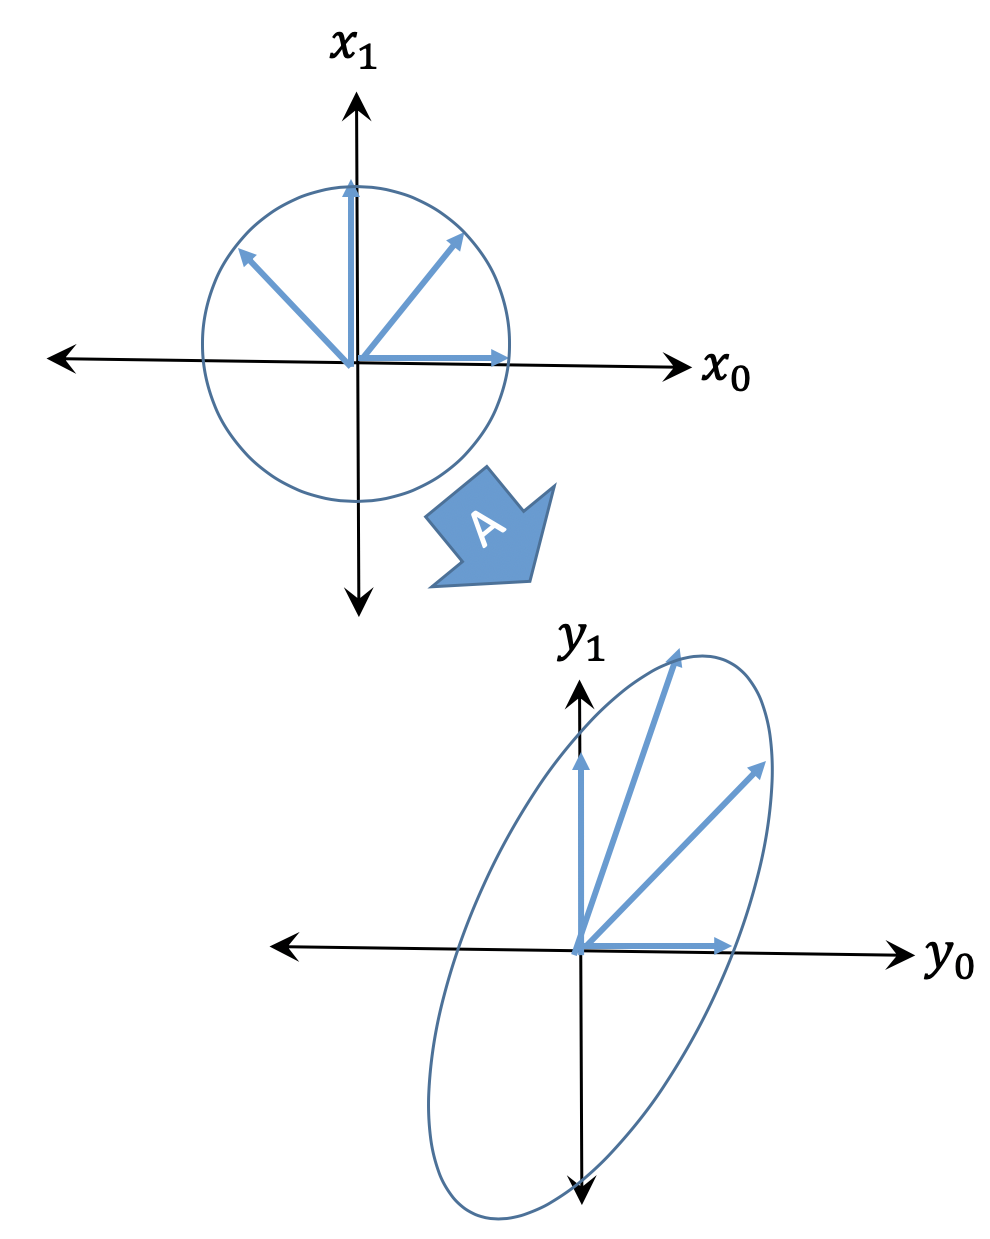
\includegraphics[width=1.45in]{linalg_review_fig1.png}
    \end{block}
  \end{columns}
\end{frame}

\begin{frame}
  \begin{columns}[t]
    \column{2.75in}
    \begin{block}{}
      A linear transform ${y}=A{x}$ maps vector
      space ${x}$ onto vector space ${y}$.  The absolute value of the
      determinant of $A$ tells you how much the area of a unit circle is
      changed under the transformation.
      
      For example, if
      $A=\left[\begin{array}{cc}1&1\\0&2\end{array}\right]$, then the
      unit circle in ${x}$ (which has an area of $\pi$) is mapped to
      an ellipse with an area that is $\mbox{abs}(|A|)=2$ times larger, i.e.,
      i.e., $\pi\mbox{abs}(|A|)=2\pi$.
    \end{block}
    \column{1.5in}
    \begin{block}{}
      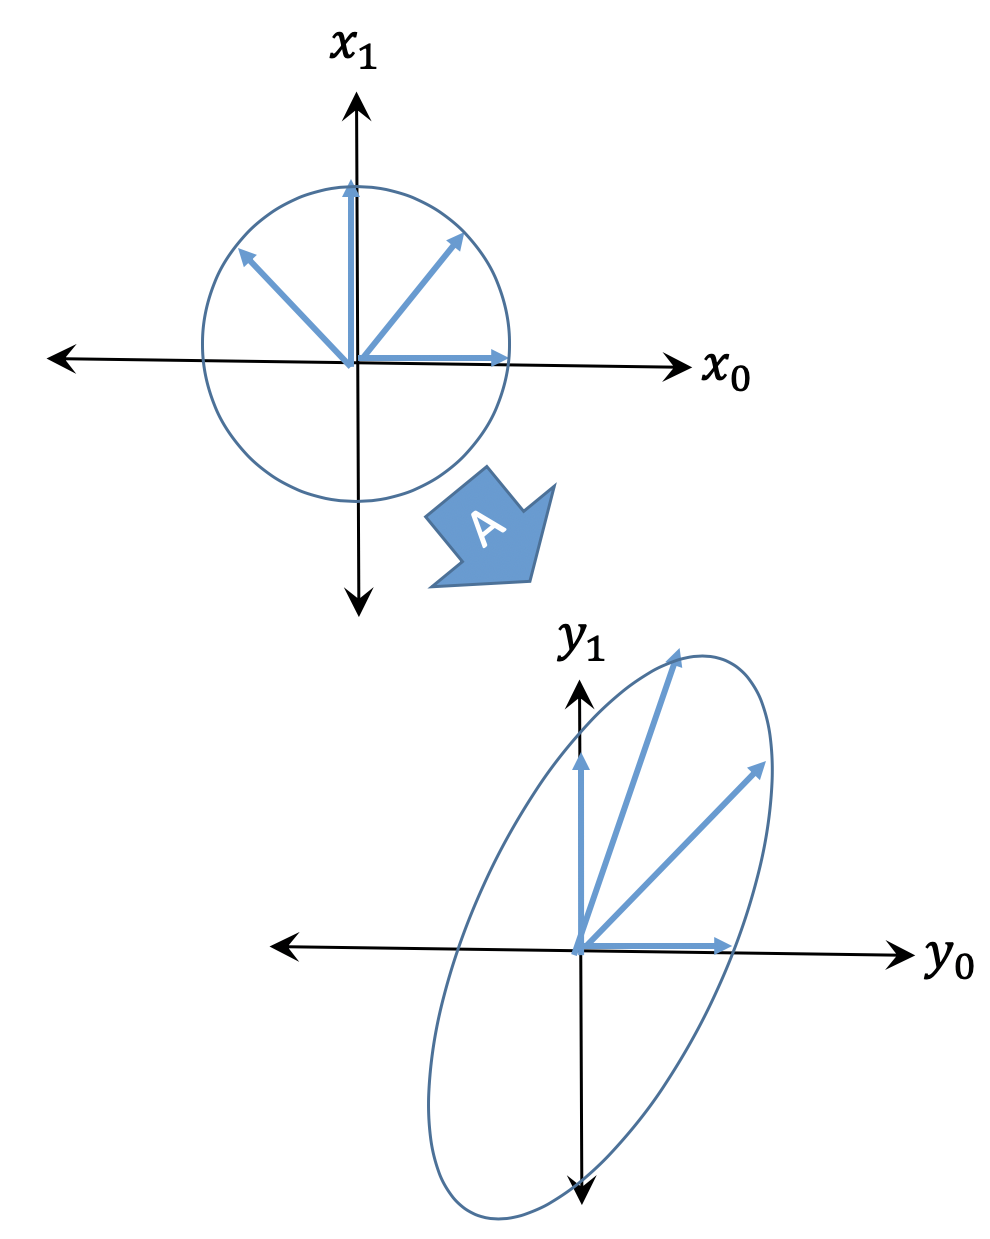
\includegraphics[width=1.45in]{linalg_review_fig1.png}
    \end{block}
  \end{columns}
\end{frame}

\begin{frame}
  \begin{columns}[t]
    \column{2.75in}
    \begin{block}{}
      For a $d$-dimensional square matrix, there may be up to $d$
        different directions ${x}={v}_i$ such that, for some
        scalar $\lambda_i$, $A{v}_i=\lambda_i{v}_i$.
        For example, if
        $A=\left[\begin{array}{cc}1&1\\0&2\end{array}\right]$, then the
        eigenvectors are
        \[
        {v}_0=\left[\begin{array}{c}1\\0\end{array}\right],~~
        {v}_1=\left[\begin{array}{c}\frac{1}{\sqrt{2}}\\\frac{1}{\sqrt{2}}\end{array}\right],~~
        \]
        and the eigenvalues are $\lambda_0=1$, $\lambda_1=2$.
        Those vectors are red and extra-thick, in the figure to the
        left.  Notice that one of the vectors gets scaled by $\lambda_0=1$, but
        the other gets scaled by $\lambda_1=2$.
    \end{block}
    \column{1.5in}
    \begin{block}{}
      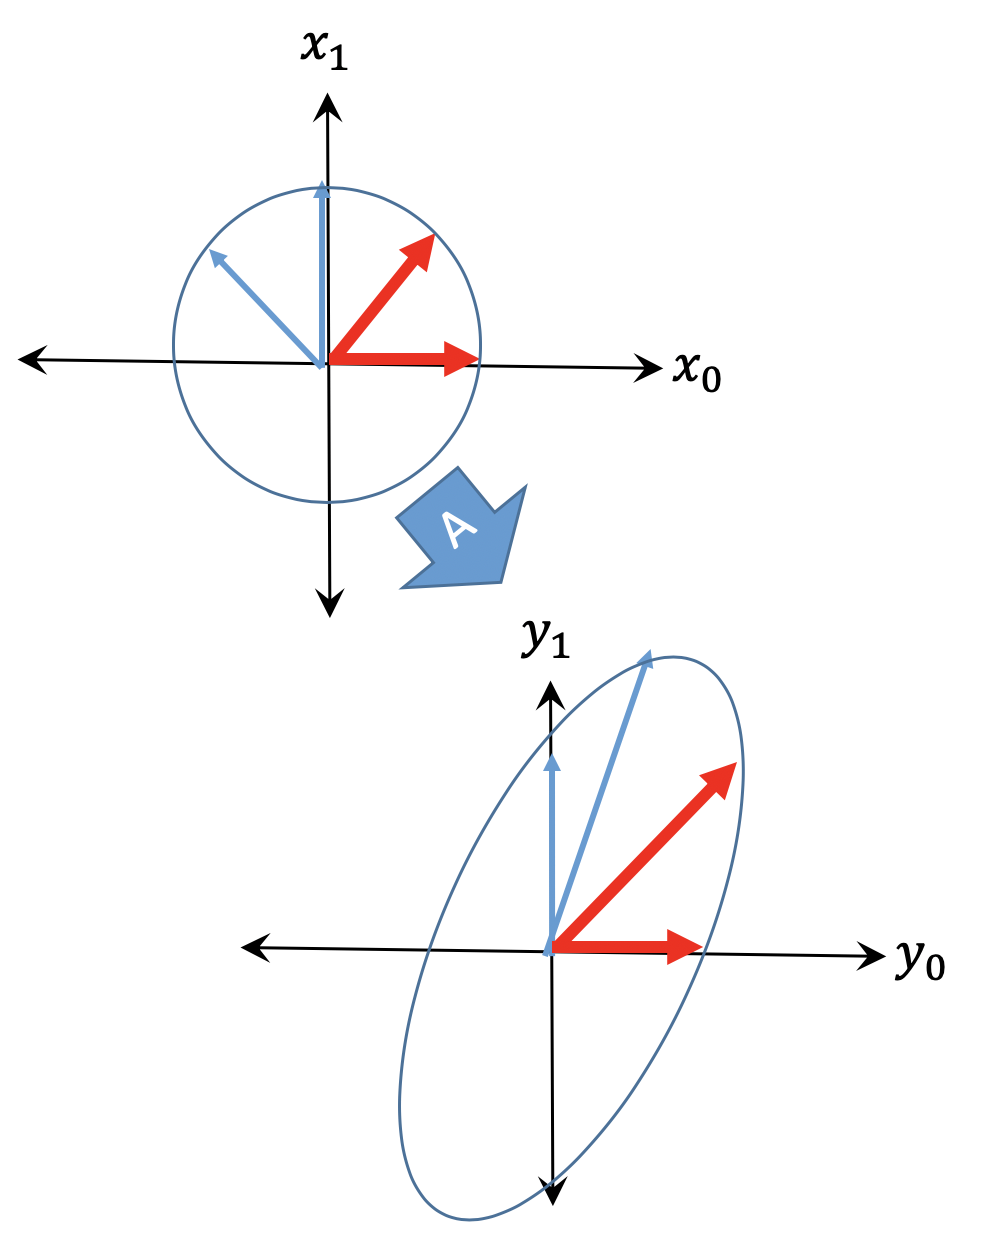
\includegraphics[width=1.45in]{linalg_review_fig2.png}
    \end{block}
  \end{columns}
\end{frame}

\begin{frame}
  \begin{columns}[t]
    \column{2.75in}
    \begin{block}{}
        An eigenvector is a direction, not just a vector.  That means
        that if you multiply an eigenvector by any scalar, you get the
        same eigenvector: if $A{v}_i=\lambda_i{v}_i$, then it’s
        also true that $cA{v}_i=c\lambda_i{v}_i$ for any scalar $c$.
        For example: the following are the same eigenvector as ${v}_1$
        \[
        \sqrt{2}{v}_1=\left[\begin{array}{c}1\\1\end{array}\right],~~
        -{v}_1=\left[\begin{array}{c}-\frac{1}{\sqrt{2}}\\-\frac{1}{\sqrt{2}}\end{array}\right]
        \]
        Since scale and sign don't matter, by convention, we normalize so that 
        an eigenvector is always unit-length ($\Vert{v}_i\Vert=1$) and
        the first nonzero element is non-negative ($v_{d,1}>0$).
    \end{block}
    \column{1.5in}
    \begin{block}{}
      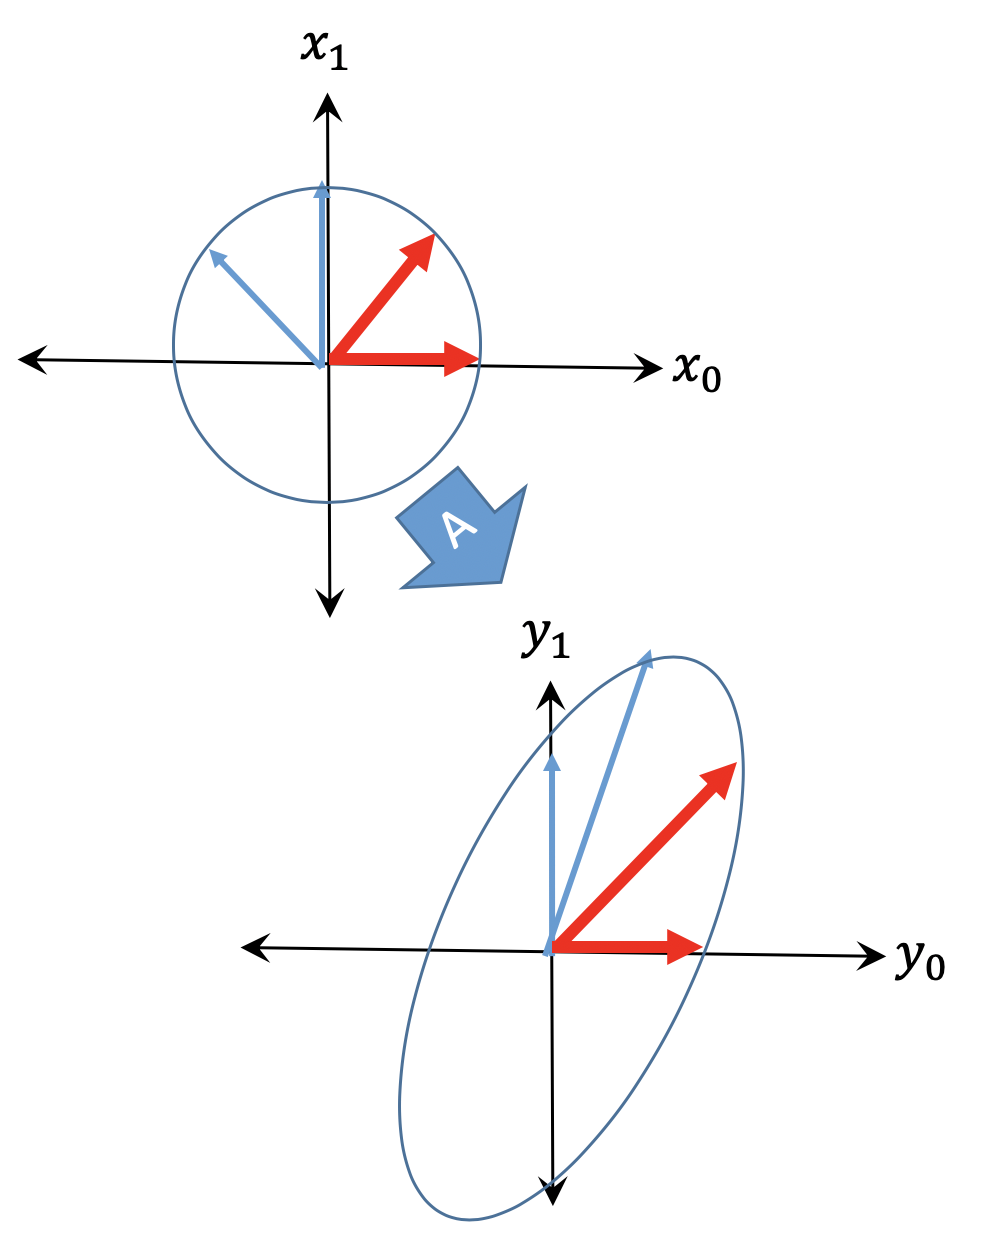
\includegraphics[width=1.45in]{linalg_review_fig2.png}
    \end{block}
  \end{columns}
\end{frame}

\begin{frame}
  \begin{columns}[t]
    \column{2.75in}
    \begin{block}{}
      \noindent{\bf Eigenvalues:}
      Before you find the eigenvectors, you should first find
      the eigenvalues.  You can do that using this fact:
      \begin{align*}
        A{v}_i &= \lambda_i{v}_i\\
        A{v}_i &= \lambda_i I{v}_i\\
        A{v}_i-\lambda_i I{v}_i &={0}\\
        (A-\lambda_i I){v}_i &= {0}
      \end{align*}
      That means that when you use the linear transform
      $(A-\lambda_i I)$ to transform the unit circle, the result has an
      area of $|A-\lambda I|=0$.
    \end{block}
    \column{1.5in}
    \begin{block}{}
      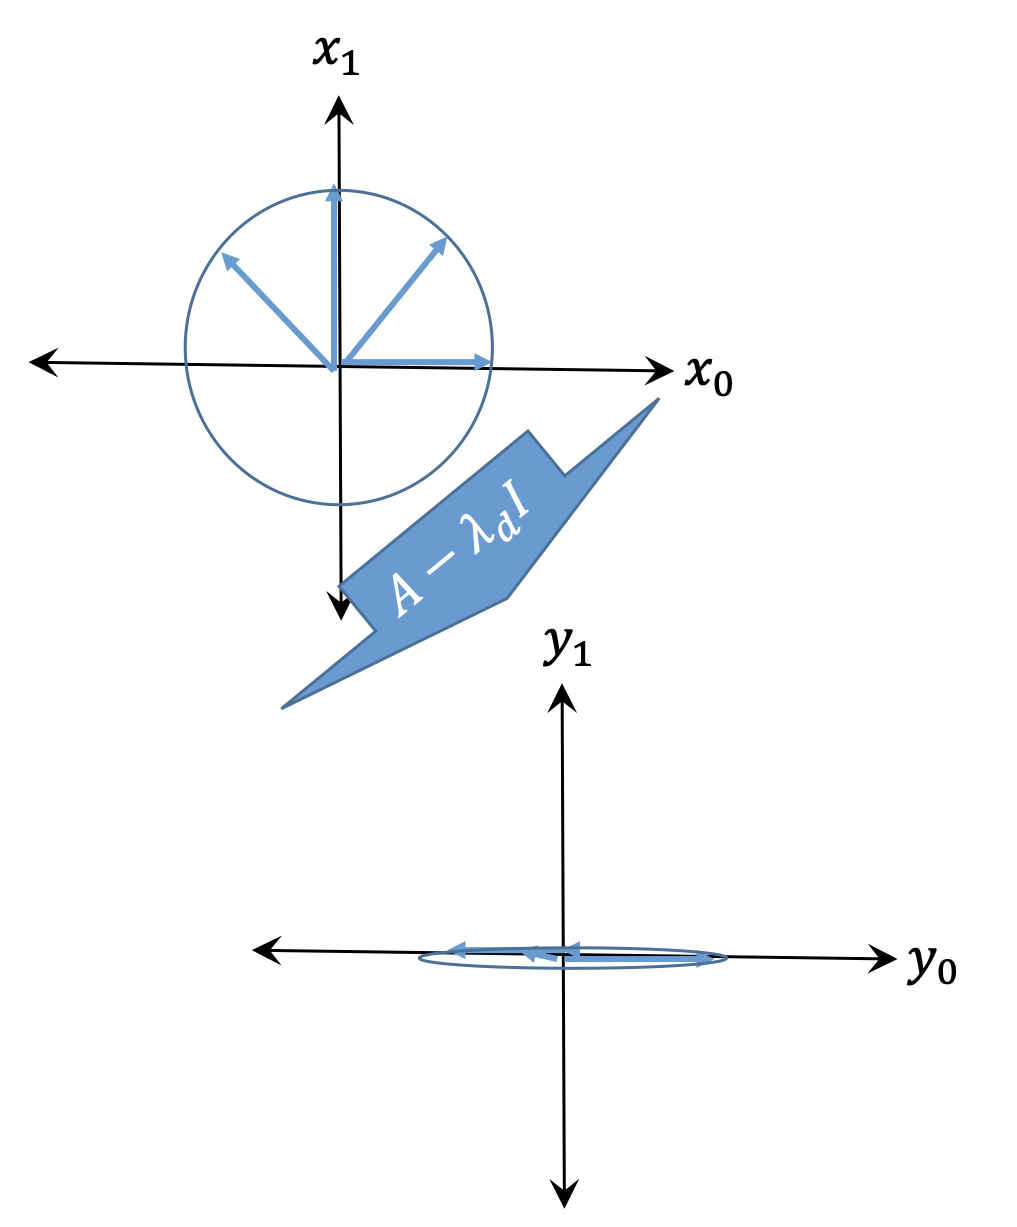
\includegraphics[width=1.45in]{linalg_review_fig3.png}
    \end{block}
  \end{columns}
\end{frame}

\begin{frame}
  \begin{columns}[t]
    \column{2.75in}
    \begin{block}{}
      \noindent{\bf Example:}
      \begin{align*}
        |A-\lambda I| &=
        \left|\begin{array}{cc}1-\lambda&1\\0&2-\lambda\end{array}\right|\\
        &=2-3\lambda+\lambda^2
      \end{align*}
      which has roots at $\lambda_0=1$, $\lambda_1=2$
    \end{block}
    \column{1.5in}
    \begin{block}{}
      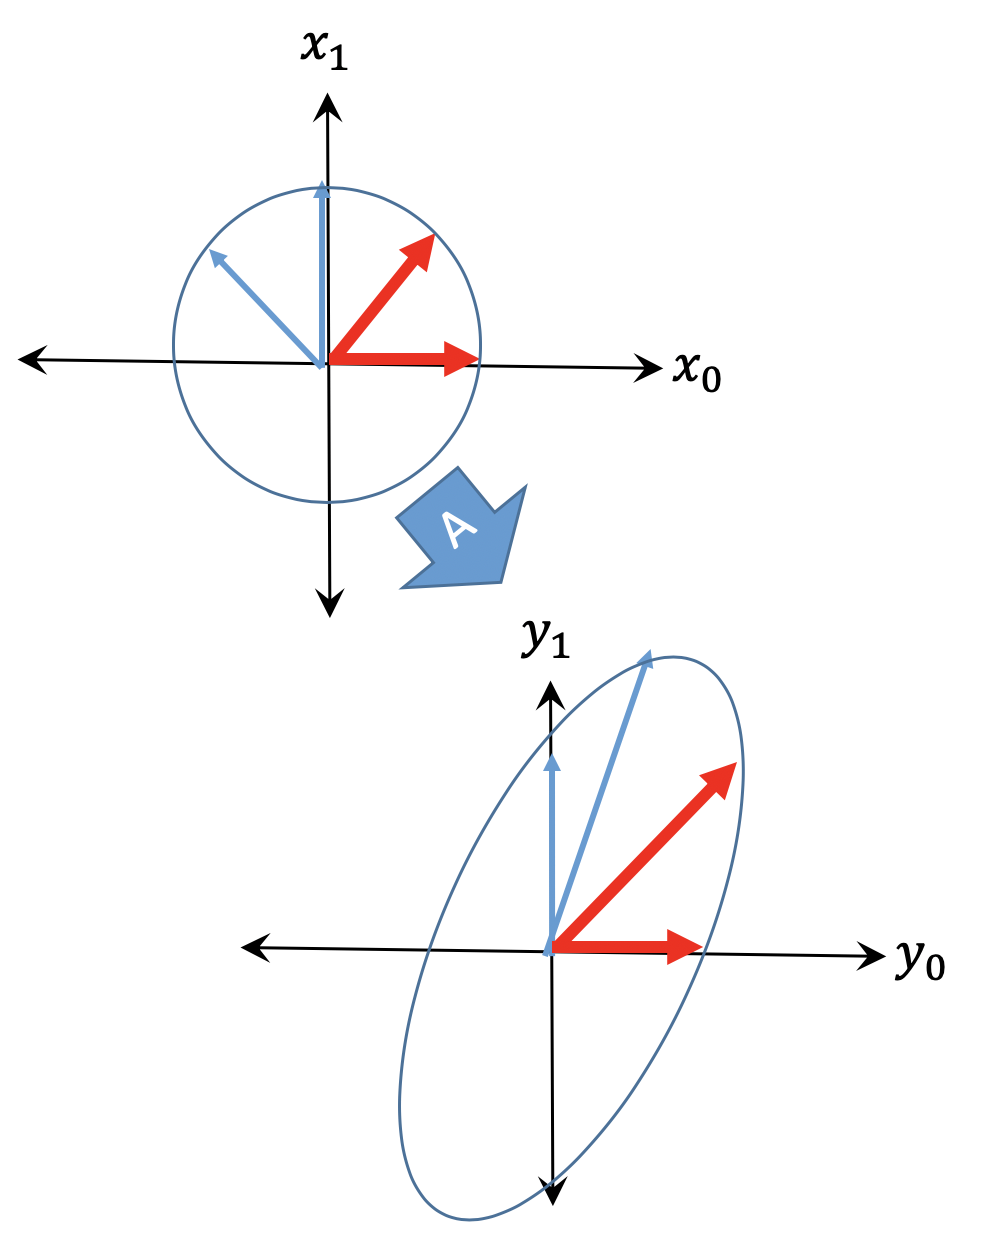
\includegraphics[width=1.45in]{linalg_review_fig2.png}
    \end{block}
  \end{columns}
\end{frame}

\begin{frame}
  \frametitle{There are always $d$ eigenvalues}
  \begin{itemize}
  \item The determinant $|A-\lambda I|$ is a $d^{\textrm{th}}$-order polynomial in $\lambda$.
  \item By the fundamental theorem of algebra, the equation
    \[
    |A-\lambda I|=0
    \]
    has exactly $d$ roots (counting repeated roots and complex roots).
  \item Therefore, {\bf any square matrix has exactly $d$ eigenvalues}
    (counting repeated eigenvalues, and complex eigenvalues).
  \end{itemize}
\end{frame}

\begin{frame}
  \frametitle{There are not always $d$ unique real eigenvectors}

  Not every square matrix has $d$ uniquely-defined, real-valued
  eigenvectors.  Some of the most common exceptions are {\bf repeated
    eigenvalues} and {\bf complex eigenvalues}.
  \begin{itemize}
  \item {\bf Repeated eigenvalues:} if two of the roots of the
    polynomial are the same ($\lambda_j=\lambda_i$), then that means
    there is a two-dimensional subspace, ${v}$, such that
    $A{v}=\lambda_i{v}$.  SOLUTION: You can arbitrarily choose any two
    orthogonal vectors from this subspace to be the eigenvectors.
    These are not uniquely defined, but you can choose a set which is
    convenient.
  \end{itemize}
\end{frame}

\begin{frame}
  \frametitle{There are not always $d$ unique real eigenvectors}

  \begin{itemize}
  \item {\bf Complex eigenvalues:} A real-valued matrix can have
    complex eigenvalues only if the corresponding eigenvectors are
    also complex.  Usually this means that there is some sort of
    periodic sinusoidal transformation of any real-valued vector.  For
    example, consider this matrix:
    \[
    A=\left[\begin{array}{cc}0&1\\-1&0\end{array}\right]
    \]
    Any real-valued vector $x=[x_1,x_2]^T$ has its elements swapped,
    i.e., $Ax=[x_2,-x_1]^T$.  However, this matrix has complex
    eigenvalues $\lambda=\pm j$, and corresponding complex
    eigenvectors such that $Av_i=\lambda_iv_i$:
    \[
    {v}_1=\frac{1}{\sqrt{2}}\left[\begin{array}{c}1\\j\end{array}\right],~~~
    {v}_2=\frac{1}{\sqrt{2}}\left[\begin{array}{c}1\\-j\end{array}\right]
    \]
   \end{itemize}
\end{frame}


%%%%%%%%%%%%%%%%%%%%%%%%%%%%%%%%%%%%%%%%%%%%%%%%%%%%%%%%%%%%%%%%%%%%%%%%%%%%%%%%%%%%%
\section[Eigenvectors]{Left and Right Eigenvectors}
\setcounter{subsection}{1}

\begin{frame}
  \frametitle{Left and right eigenvectors}
  We’ve been working with right eigenvectors and right eigenvalues: 
  \[
  A{v}_i =\lambda_i{v}_i
  \]
  There may also be left eigenvectors, which are row vectors ${u}_i$
  and corresponding left eigenvalues $\kappa_i$:
  \[
  {u}_i^T A = \kappa_i{u}_i^T
  \]
  It turns out that (1) the eigenvalues are the same,
  $\kappa_i=\lambda_i$, (2) the eigenvectors might not be the same, but
  (3) unpaired eigenvectors are orthogonal.
\end{frame}

\begin{frame}
  \frametitle{Proof: Right \& Left Eigenvalues are the same}
  You can do an interesting thing if you multiply the matrix by its eigenvectors both before and after:
  \[
  {u}_i^T(A{v}_j)={u}_i^T(\lambda_j{v}_j)=\lambda_j{u}_i^T{v}_j
  \]
  \ldots but\ldots
  \[
  ({u}_i^TA){v}_j=(\kappa_i{u}_i^T){v}_j=\kappa_i{u}_i^T{v}_j
  \]
  There are only two ways that both of these things can be true. Either
  \[
  \kappa_i=\lambda_j~~~\mbox{or}~~~{u}_i^T{v}_j=0
  \]
\end{frame}

\begin{frame}
  \frametitle{Summary: Left and right eigenvalues must be paired!!}

  Summary: for an arbitrary square matrix $A$,
  \begin{itemize}
  \item Left and right eigenvalues are the same,
    $\lambda_i=\kappa_i\forall i$.
  \item Eigenvectors might NOT be the same
  \item Left and right eigenvectors of unpaired eigenvalues are
    orthogonal, $\lambda_i\ne\lambda_j \Rightarrow u_i^Tv_j=0$.
  \end{itemize}
\end{frame}

%%%%%%%%%%%%%%%%%%%%%%%%%%%%%%%%%%%%%%%%%%%%
\section[Symmetric]{Symmetric PSD Matrices}
\setcounter{subsection}{1}

%\begin{frame}
%  \frametitle{Properties of symmetric matrices}
%  If $A$ is symmetric with $d$ eigenvectors, and $d$ distinct eigenvalues, then
%  \[
%  VV^T=V^TV=I
%  \]
%  \[
%  V^TAV = \Lambda
%  \]
%  \[
%  A=V\Lambda V^T
%  \]
%\end{frame}

\begin{frame}
  \frametitle{Symmetric matrices: left=right}

  Suppose that $A$ is any arbitrary matrix, not even square.  The
  product $AA^T$ is both square and symmetric.  For example:
  \begin{align*}
    AA^T &= \left[\begin{array}{ccc}a_{1,1}&a_{1,2}&a_{1,3}\\a_{2,1}&a_{2,2}&a_{2,3}\end{array}\right]
    \left[\begin{array}{cc}a_{1,1}&a_{2,1}\\a_{1,2}&a_{2,2}\\a_{1,3}&a_{2,3}\end{array}\right]\\
    &=
    \left[\begin{array}{cc}\sum_ja_{1,j}^2&\sum_ja_{1,j}a_{2,j}\\\sum_ja_{1,j}a_{2,j}&\sum_ja_{2,j}^2
      \end{array}\right]
  \end{align*}
\end{frame}

\begin{frame}
  \frametitle{Positive semi-definite matrices}

  The matrix $AA^T$ is also positive semi-definite ($AA^T\succeq 0$),
  meaning that
  \begin{itemize}
  \item Its determinant is non-negative, $\mbox{det}(AA^T)\ge 0$, and
  \item all of its eigenvalues are non-negative, $\lambda_i \ge 0$.
  \end{itemize}
  Intuitive explanation (not quite a proof): suppose
  $A=[a_1,\ldots,a_m]^T$.  Then the elements on the main diagonal are
  larger than the other elements in the sense that
  \begin{align*}
    a_i^Ta_j &= \Vert a_i\Vert\cdot\Vert a_j\Vert\cos\left(\angle(a_i,a_j)\right)\le\Vert a_i\Vert\cdot
    \Vert a_j\Vert
  \end{align*}
\end{frame}

\begin{frame}
  \frametitle{Symmetric matrices: left=right}

  Suppose $\Sigma=AA^T$ is any symmetric square matrix: then its left
  and right eigenvectors and eigenvalues are the same.
  \begin{itemize}
  \item The right eigenvectors are $\lambda_iv_i=\Sigma v_i$
  \item The left eigenvectors are $\lambda_i u_i^T = u_i^T \Sigma$
  \item \ldots but transposing $\Sigma v_i$ gives:
    \[
    (\Sigma v_i)^T = v_i^T\Sigma^T = v_i^T\Sigma
    \]
    \ldots so it must be the case that $v_i=u_i$.
  \end{itemize}
\end{frame}

\begin{frame}
  \frametitle{Positive semidefinite (PSD) matrices: real generalized eigenvectors}

  Suppose $\Sigma=AA^T\succeq 0$.  Then every eigenvalue has an
  associated generalized eigenvector:
  \begin{itemize}
  \item If $\lambda_i$ is unique, then there is an associated real
    eigenvector, $\lambda_iv_i = \Sigma v_i$.
  \item If $\lambda_i=\lambda_{i+1}=\cdots \lambda_{i+k=1}$, then
    there is a $k$-dimensional subspace whose vectors $v$ all satisfy
    $\lambda_iv =\Sigma v$.  We can choose an arbitrary
    orthonormal basis of that subspace, and call those the
    ``generalized eigenvectors'' $v_i,\cdots,v_{i+k-1}$ of
    $\lambda_i,\cdots,\lambda_{i+k-1}$.
    \begin{itemize}
    \item 
      Most common example: if $A\in\Re^{mxn},n>m$, then at least $n-m$
      of the eigenvalues of $\Sigma$ are zero.
    \end{itemize}
  \end{itemize}
\end{frame}

\begin{frame}
  \frametitle{Symmetric matrices: eigenvectors are orthonormal}
  Let's combine the following facts:
  \begin{itemize}
  \item ${u}_i^T{v}_j=0$ for $i\ne j$ --- any square matrix with distinct
    eigenvalues
  \item ${u}_i={v}_i$ --- symmetric matrix
  \item ${v}_i^T{v}_i=1$ --- standard normalization of
    eigenvectors for any matrix (this is what $\Vert{v}_i\Vert=1$ means).
  \end{itemize}
  Putting it all together, we get that
  \[
  {v}_i^T{v}_j=
  \begin{cases}
    1&i=j\\
    0&i\ne j
  \end{cases}
  \]
\end{frame}

\begin{frame}
  \frametitle{The eigenvector matrix}
  So if $\Sigma$ is symmetric with distinct eigenvalues, then
  its eigenvectors  are orthonormal:
  \[
  {v}_i^T{v}_j=
  \begin{cases}
    1&i=j\\
    0&i\ne j
  \end{cases}
  \]
  We can  write this as
  \[
  V^TV = I
  \]
  where
  \[
  V=\left[{v}_1,\ldots,{v}_{d}\right]
  \]
\end{frame}

\begin{frame}
  \frametitle{The eigenvector matrix is orthonormal}
  \[
  V^TV = I
  \]
  \ldots and it also turns out that
  \[
  VV^T = I
  \]
\end{frame}

\begin{frame}
  \frametitle{Eigenvectors orthogonalize a symmetric matrix}
  \[
  {v}_i^T\Sigma{v}_j=
  {v}_i^T(\lambda_j{v}_j)=\lambda_j{v}_i^T{v}_j
  =\begin{cases}\lambda_j,&i=j\\0,&i\ne j\end{cases}
  \]
  In other words, if a symmetric matrix has $d$ eigenvectors with
  distinct eigenvalues, then its eigenvectors orthogonalize it:
  \[
  V^T\Sigma V = \Lambda
  \]
  \[
  \Lambda=
  \left[\begin{array}{ccc}\lambda_1&0&0\\0&\ldots&0\\0&0&\lambda_{d}\end{array}\right]
  \]
\end{frame}

\begin{frame}
  \frametitle{Summary: symmetric positive semi-definite matrices}

  If $\Sigma$ is symmetric and positive semi-definite, then
  \[
  \Lambda = V^T\Sigma V
  \]
  \[
  VV^T=V^TV=I
  \]
  Putting those two together, we also get this statement, which says
  that you can reconstruct $\Sigma$ from the scaled outer products of
  its eigenvectors:
  \[
  V\Lambda V^T = VV^T\Sigma VV^T = \Sigma
  \]
\end{frame}

%%%%%%%%%%%%%%%%%%%%%%%%%%%%%%%%%%%%%%%%%%%%%%%%%%%%%%%%%%%%%%%%%%%%%%%%%%%%%%%%%%%%%
\section{Examples}
\setcounter{subsection}{1}

\begin{frame}
  \frametitle{In-Lecture Written Example Problem}
  
  Pick an arbitrary $2\times 2$ symmetric matrix.  Find its
  eigenvalues and eigenvectors.  Show that $\Lambda=V^TAV$ and
  $A=V\Lambda V^T$.
\end{frame}
  
\begin{frame}
  \frametitle{In-Lecture Jupyter Example Problem}
  
  Create a jupyter notebook.  Pick an arbitrary $2\times 2$ matrix.
  Plot a unit circle in the ${x}$ space, and show what happens to
  those vectors after transformation to the ${y}$ space.
  Calculate the determinant of the matrix, and its eigenvalues and
  eigenvectors.  Show that $A{v}=\lambda{v}$.
  
\end{frame}
  
%%%%%%%%%%%%%%%%%%%%%%%%%%%%%%%%%%%%%%%%%%%%%%%%%%%%%%%%%%%%%%%%%%%%%%%%%%%%%%%%%%%%%
\section{Summary}
\setcounter{subsection}{1}

\begin{frame}
  \frametitle{Summary}
  \begin{itemize}
  \item A linear transform, $A$, maps vectors in space ${x}$ to vectors in space ${y}$.
  \item The determinant, $|A|$, tells you how the volume of the unit
    sphere is scaled by the linear transform.
  \item Every $d\times d$ linear transform has $d$ eigenvalues, which
    are the roots of the equation $|A-\lambda I|=0$.
  \item Left and right eigenvectors of a matrix are either orthogonal
    (${u}_i^T{v}_j=0$) or share the same eigenvalue ($\kappa_i=\lambda_j$).
  \item For a symmetric positive semidefinite matrix $\Sigma =AA^T$,
    the left and right eigenvectors are the same.  If the eigenvalues
    are distinct and real, then:
    \[
    \Sigma=V\Lambda V^T,~~~\Lambda = V^T\Sigma V,~~~VV^T=V^TV=I
    \]
  \end{itemize}
\end{frame}


\end{document}

